\section{Optimal Block Size} \label{sec:res-blocksize}

% TODO make concrete suggestions for optimal block size (table maybe?)

% \begin{table}
%     \begin{tabular}{l p{2.35cm} p{2.35cm} p{2.35cm} p{2.35cm}}
%         \hline
%         Access & {\raggedright chasing, uncompressed} & {\raggedright non-chasing, uncompressed} & {\raggedright chasing, compressed} & {\raggedright non-chasing, compressed} \\
%         \hline
%         \hline
%         hdiff & & & & \\
%         \emph{naive} & $32\times 1\times 8$ & $64\times 1\times 8$ & $256\times 1\times 1$ & $128\times 1\times 2$ \\
%         \emph{idxvar} & $64\times 1\times 8$ & $32\times 1\times 16$ & $128\times 1\times 2$ & $64\times 1\times 2$ \\
%     \end{tabular}
% \end{table}

One of the main determining factors for the performance of a kernel is the launch configuration, which includes grid size (number of blocks) and block size (number of threads, described in section \ref{sec:hardware}). As we implemented and evaluated our grid storage and grid access strategies, we consistently ran our benchmarks across a large range of launch configurations. In the previous sections, we reported best-case runtimes using the respective optimal launch configuration. This optimal configuration varies heavily depending on the implementation, as we will detail in this section.

CUDA provides the option to specify block sizes in three dimensions, providing each thread with an X-, Y- and Z-index. In our benchmarks, we have tested all possible combinations of block sizes in steps of powers of two from $32$ up to $512$. In order to cover the entire problem domain (which remains constant in size), a decrease in the number of threads is always accompanied by an increase in the number of blocks (grid size) and vice versa. Owing to the way we map thread indices onto memory indices (X thread index maps onto memory index directly), thread sizes in the X-dimension of less than $32$ are highly inefficient, as they lead to non-coalescing memory accesses. The X-dimension of the benchmarked block sizes is therefore always at least $32$.

\subsection{Overview}

\begin{figure}
	\begin{center}
    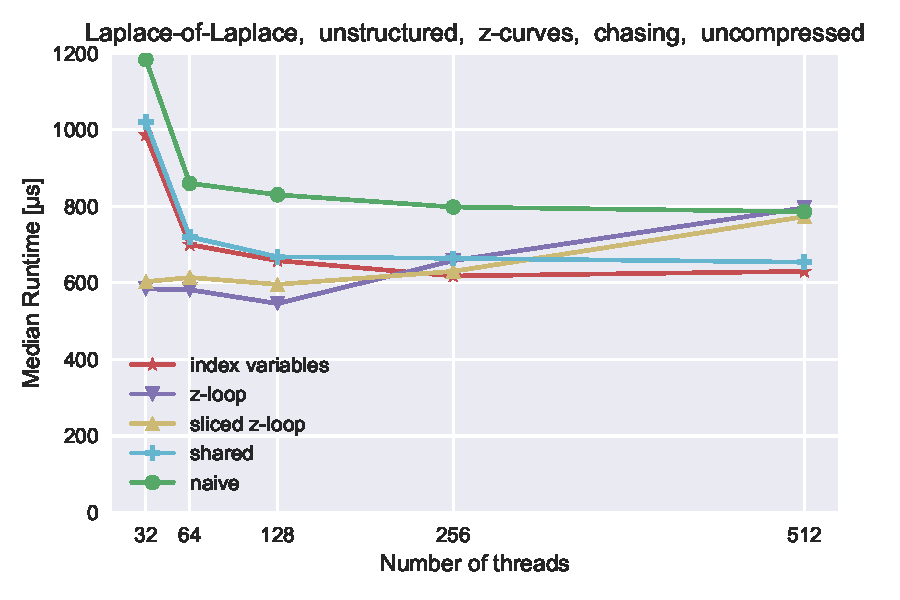
\includegraphics[scale=0.75]{threads-total-laplap.pdf}
	\end{center}
    \caption{\label{fig:blocksizes-overview} Impact of the total number of threads on the runtime for different implementations of the \emph{laplap} stencil ($512\times 512\times 64$ grid, \emph{z-curves} memory layout with \emph{double} precision, \emph{chasing} and \emph{uncompressed} neighborship table). }%The low-occupancy \emph{z-loop} and \emph{z-loop-sliced} access strategies do not profit from a larger number of threads, contrary to the other variants. Results for other stencils and variants are of similar shape.}
% >>> u.lineplot(df[(df["size-z"]==64)&(df["stencil"]=="laplap")&df["z-curves"]&~df["no-chase"]&~df["comp"]], x="threads-prod", y="median")
% >>> plt.ylabel("Median Runtime [µs]")
% Text(0, 0.5, 'Median Runtime [µs]')
% >>> plt.ylim(0, 1200)
% (0, 1200)
% >>> plt.grid("both")
% >>> fig=u.plotdone(legend=0)
% >>> u.plotsave("report/img/threads-total-laplap.pdf", fig)
\end{figure}

The optimal \emph{total number} of threads depends mostly on the grid access implementation employed. In general, the same patterns can be observed for all three tested stencils and all tested grid memory storage implementations: When using the \emph{naive}, \emph{idxvar} or \emph{shared} grid access strategies, it is best to have a high number of threads in total ($256-512$). The \emph{z-loop} and \emph{z-loop-sliced} thrive on a lower number of threads due to occupancy concerns. An exemplary overview of the runtimes as a function of total block size is given in figure \ref{fig:blocksizes-overview}.

\begin{figure}
	\begin{center}
    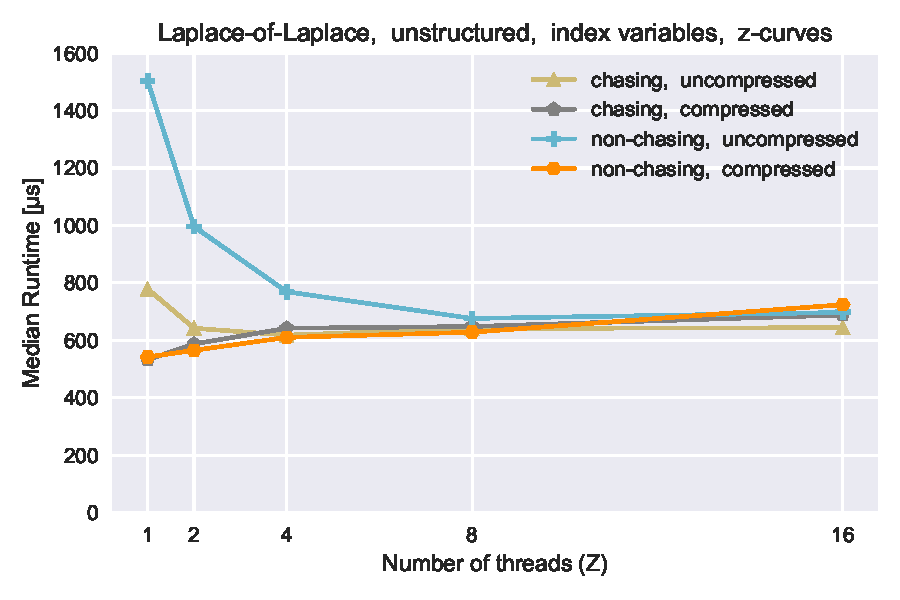
\includegraphics[scale=0.75]{threads-z-storages.pdf}
% >>> u.lineplot(df[(df["size-z"]==64)&(df["stencil"]=="laplap")&df["z-curves"]&df["unstructured"]&(df["variant"]=="idxvar")],by=["no-chase", "comp"], x="threads-z", y="median")
% >>> plt.ylabel("Median Runtime [µs]")
% Text(0, 0.5, 'Median Runtime [µs]')
% >>> plt.grid("both")
% >>> plt.ylim(0, 1600)
% (0, 1600)
% >>> fig=u.plotdone(legend=0)
% >>> u.plotsave("report/img/threads-z-storages.pdf", fig)
	\end{center}
    \caption{\label{fig:blocksizes-z}Fastest runtimes of all configurations for fixed numbers of threads in the Z-dimension (other dimensions free) for the \emph{laplap} stencil ($512\times 512\times 64$ grid, \emph{row-major} memory layout with \emph{double} precision). Note how the Z-regularity of the grid makes it advantageous to have a larger number of threads in the Z-dimension, as this leads to caching of neighborship table entries, but only if the neighborship table is \emph{uncompressed}.}
\end{figure}

The best \emph{shape} of the block size vector changes with the used grid storage strategy. Using \emph{uncompressed} neighborship tables, it is best for the \emph{naive}, \emph{idxvar} and \emph{shared} access strategies to have $32$ or $64$ threads in X-dimension and the rest in Z-dimension. Those implementations profit of more Z-threads because of the regularity of the grid in the Z-dimension. The \emph{non-chasing} variants profit even more of additional threads in the Z-dimension. This is because, in non-chasing variants, more neighborships are stored in the table; cache entries are thus evicted faster if many different X- and Y-coordinates are accessed. In \emph{compressed} neighborship tables, on the other hand, additional threads in the Z-dimension are of no use to any of the access strategies -- the greatly reduced number of neighborship table entries after compression remains in cache independent of the Z-block-size. See figure \ref{fig:blocksizes-z} for a comparison of how changes in the Z-dimension of the block size vector translate to runtime changes. Whether the grid is stored as \emph{row-major} or using \emph{z-order} curves does not strongly impact the required block sizes.

\subsection{Optimal Block Sizes per Access Strategy}

In this section, we further elaborate on the optimal block sizes for each access strategy and aim to explain (using profiler metrics) why certain shapes of thread blocks are beneficial.

\subsubsection{\emph{Naive}, \emph{Idxvar} and \emph{Shared} Grid Access Strategies}

In order to always cover the entire problem domain, the number of blocks $b$ in each dimension in the \emph{naive}, \emph{idxvar} and \emph{shared} grid access strategies is chosen as a function on the problem size $d$ and the chosen number of threads $t$ as follows:
$$b = \begin{pmatrix}\left\lceil\frac{d_x}{t_x}\right\rceil & \left\lceil\frac{d_y}{t_y}\right\rceil & \left\lceil\frac{d_z}{t_z}\right\rceil\end{pmatrix}^\top$$

For the \emph{naive}, \emph{idxvar} and \emph{shared} implementations, a high total number of threads per block is beneficial to performance. For grids using an \emph{uncompressed} neighborship table, increasing the number of threads in the Z-dimension especially improves performance.

\begin{table}
%    \begin{tabular}{l l l l l}
%        Blocksize & \texttt{global\_hit\_rate} & \texttt{tex\_cache\_hit\_rate} & \texttt{l2\_tex\_read\_hit\_rate} & \texttt{l2\_tex\_hit\_rate} \\
%        \hline
%        $32\times 1\times 1$ & $45.42\%$ & $44.39\%$ & $73.86\%$ & $67.69\%$ \\
%        $32\times 1\times 2$ & $58.83\%$ & $57.96\%$ & $76.60\%$ & $68.12\%$ \\
%        $64\times 1\times 2$ & $62.25\%$ & $66.21\%$ & $69.99\%$ & $60.36\%$ \\
%        $64\times 1\times 4$ & $72.33\%$ & $71.72\%$ & $72.77\%$ & $60.81\%$
%    \end{tabular}
	\begin{center}
    \begin{tabular}{l l l p{2cm} p{2cm}}
        \hline
        \textbf{Blocksize} & \textbf{\texttt{tex\_\allowbreak cache\_\allowbreak hit\_\allowbreak rate}} & \textbf{\texttt{l2\_\allowbreak tex\_\allowbreak hit\_\allowbreak rate}} \\
        \hline
        \hline
        $32\times 1\times 1$ & $44.39\%$ & $67.69\%$ \\
        $32\times 1\times 2$ & $57.96\%$ & $68.12\%$ \\
        $64\times 1\times 2$ & $66.21\%$ & $60.36\%$ \\
        $64\times 1\times 4$ & $71.72\%$ & $60.81\%$ \\
        \hline
    \end{tabular}
	\end{center}
    \caption{\label{tab:laplap-blocksize-metrics} Cache hit rates for different block sizes for the \emph{laplap} stencil, implemented using a \emph{idxvar} grid access strategy on a $512\times 512\times 64$-sized domain (\emph{z-curves} memory layout with \emph{double} precision, \emph{chasing} and \emph{uncompressed} neighborship table).}
\end{table}

For the \emph{naive} and \emph{idxvar} strategies (in grids using uncompressed neighborship tables), the advantage of multiple Z-threads can be explained through the regularity of the grid in the Z-dimension. Threads operating on cells with identical X- and Y-coordinates access the neighborship tables at the \emph{same index}. When multiple threads operate on different Z-levels, caching of these shared neighborship table entries becomes very effective. Evidence for this presumed reason for the speedup is given by two facts: One, of all block size combinations tested, the ones with more threads in the Z-dimension perform best. Two, the Nvidia profiler reports higher cache hit rates if the number of threads in Z-dimension is increased. As an example of this for the \emph{idxvar} access strategy, see table \ref{tab:laplap-blocksize-metrics}.

These effects are strongest when using \emph{non-chasing} grid storage. As this type of storage leads to a larger number of entries in the neighborship table, entries may be evicted from the cache more quickly. More threads in the Z-dimension, which access the same neighborship table entries, prevent this by keeping the relevant neighborship table entries ``fresh.''

At the opposite end of the spectrum lie the grids stored using \emph{compressed} neighborship tables. These tables are much smaller, and the same few entries are accessed in almost all threads. Because of this, neighborship table entries remain in cache no matter what the shape of the block size vector is, and additional threads in the Z-dimension bring no benefit. Cache locality for the accessed values is more important here; depending on the used layout for the values (\emph{z-curves} or \emph{row-major}) this means adding additional threads in X (\emph{z-curves}, spatial locality given), or X and Y (\emph{row-major}, adding another thread in Y gives some spatial locality).

By the design of the \emph{shared} access strategy, a speedup is supposed to be attained with a larger number of Z-threads; if there are more threads in Z-dimension within a block, more sharing of neighborship relations through shared memory can take place. These implementations indeed profit from more threads through shared memory in much the same way as \emph{naive} and \emph{idxvar} variants profit from more threads through the cache in the uncompressed grids.

\subsubsection{\emph{Z-loop} and \emph{Z-loop-sliced} Grid Access Strategies}

\begin{table}
	\begin{center}
    \begin{tabular}{l l l p{2.5cm} p{2.5cm}}
        \hline
        \textbf{Variant} & \textbf{Blocksize} & \textbf{Runtime} & \textbf{\texttt{achieved\_\allowbreak occupancy}} & \textbf{\texttt{issue\_\allowbreak slot\_\allowbreak utilization}} \\
        \hline
        \hline
        \emph{idxvar} & $512$ & $783\mu s$ & $85\%$ & $19\%$ \\
        \emph{idxvar} & $128$ & $844\mu s$ & $\mathbf{92\%}$ & $18\%$ \\
        \emph{idxvar} & $32$  & $986\mu s$ & $48\%$ & $16\%$ \\
        \emph{z-loop} & $512$ & $796\mu s$ & $25\%$ & $10\%$\\
        \emph{z-loop} & $128$ & $\mathbf{546\mu s}$ & $42\%$ & $13\%$ \\ 
        \emph{z-loop} & $32$  & $584\mu s$ & $41\%$ & $12\%$ \\
        \hline
    \end{tabular}
	\end{center}
    \caption{\label{tab:laplap-blocksize-occupancy} Runtimes and occupancy metrics of \emph{idxvar} and \emph{z-loop} implementations of the \emph{laplap} stencil on an unstructured grid (size $512\times 512\times 64$, \emph{z-curves} memory layout with \emph{double} precision, \emph{chasing} and \emph{uncompressed} neighborship table) for a selection of block sizes. The following block shapes were used: $512 = 256\times 2\times 1$, $128 = 64\times 2\times 1$ and $32 = 32\times 1 \times 1$. This table highlights the occupancy issues the \emph{z-loop} variant faces with too large block sizes. Note how the occupancy drops with an increased number of threads, and how the runtime increases with it.}
\end{table}

Contrary to the other stencils, the \emph{z-loop} and \emph{z-loop-sliced} grid access strategies suffer from a high total thread count. As both of these strategies require one thread to perform calculations for multiple cells on different Z-levels, the total number of blocks and threads required to cover the entire grid is smaller. On the largest tested grid size ($512\times 512\times 64$), this leads to occupancy issues: As threads stall, there is not enough work that can be scheduled to certain streaming multiprocessors to hide the latency. All threads inside a block are required to be executed on the same SM; having more threads inside a block thus gives fewer blocks that can be scheduled onto stalled SMs. Smaller block sizes, on the other hand, give the scheduler a larger pool of blocks to choose from when trying to hide latency. Compare table \ref{tab:laplap-blocksize-occupancy} for an example of how a too large block size negatively impacts the \emph{z-loop} implementation of the exemplary \emph{laplap} benchmark.